\section*{Лекция 9 (14.04.2022)}
\begin{enumerate}
    \item[1] $L$ -- афинное множество. $L = L_0 + a$, где $L_0$ -- линейное множество, $a \in H$.\\
    $L = \{l + a \mid l \in L_0\}$

    %
    \tikzset{every picture/.style={line width=0.75pt}} %set default line width to 0.75pt

    \begin{tikzpicture}[x=0.75pt,y=0.75pt,yscale=-1,xscale=1]
        %uncomment if require: \path (0,300); %set diagram left start at 0, and has height of 300

        %Shape: Ellipse [id:dp5594136254073829]
        \draw   (284.61,95.02) .. controls (249.48,72.92) and (236.85,55) .. (256.39,55) .. controls (275.94,55) and (320.27,72.92) .. (355.39,95.02) .. controls (390.52,117.13) and (403.15,135.05) .. (383.61,135.05) .. controls (364.06,135.05) and (319.73,117.13) .. (284.61,95.02) -- cycle ;
        %Straight Lines [id:da5192526291436679]
        \draw    (320,95.02) -- (259,165.05) ;
        \draw [shift={(259,165.05)}, rotate = 131.06] [color={rgb, 255:red, 0; green, 0; blue, 0 }  ][fill={rgb, 255:red, 0; green, 0; blue, 0 }  ][line width=0.75]      (0, 0) circle [x radius= 3.35, y radius= 3.35]   ;
        \draw [shift={(320,95.02)}, rotate = 131.06] [color={rgb, 255:red, 0; green, 0; blue, 0 }  ][fill={rgb, 255:red, 0; green, 0; blue, 0 }  ][line width=0.75]      (0, 0) circle [x radius= 3.35, y radius= 3.35]   ;
        %Shape: Ellipse [id:dp6088740304242628]
        \draw   (201.24,163.02) .. controls (121.84,125.46) and (85.58,95) .. (120.25,95) .. controls (154.93,95) and (247.4,125.46) .. (326.8,163.02) .. controls (406.19,200.59) and (442.45,231.05) .. (407.78,231.05) .. controls (373.11,231.05) and (280.64,200.59) .. (201.24,163.02) -- cycle ;
        %Straight Lines [id:da35141840892191256]
        \draw    (100,121) ;


        % Text Node
        \draw (401,187) node [anchor=north west][inner sep=0.75pt]   [align=left] {$\displaystyle L_{0}$};
        % Text Node
        \draw (366,86) node [anchor=north west][inner sep=0.75pt]   [align=left] {$\displaystyle L$};
        % Text Node
        \draw (272,160) node [anchor=north west][inner sep=0.75pt]   [align=left] {$\displaystyle O$};

    \end{tikzpicture}

    $f(x) = \norm{x_0 - x}^2$, $x_0 \in L_0$\\
    $y_0$ -- точка минимума, необходимое условие точки минимума -- $x_0 - y_0 \perp L_0$\\
    $df(y_0) \colon L_0 \to \R$, $L_0$ -- множество допустимых приращений.

\end{enumerate}

\subsection{Задача о брахистохроне}

Брахистохрон -- кривая наибыстрейшего спуска.

\tikzset{every picture/.style={line width=0.75pt}} %set default line width to 0.75pt

\begin{tikzpicture}[x=0.75pt,y=0.75pt,yscale=-1,xscale=1]
    %uncomment if require: \path (0,300); %set diagram left start at 0, and has height of 300

    %Shape: Axis 2D [id:dp8073589947581048]
    \draw  (44.39,13) -- (44.39,253.06)(378,35.76) -- (17,35.76) (49.39,246.06) -- (44.39,253.06) -- (39.39,246.06) (371,30.76) -- (378,35.76) -- (371,40.76)  ;
    %Curve Lines [id:da7700543933609254]
    \draw    (45,39) .. controls (66.12,145.35) and (171.39,208.78) .. (309,181.06) ;
    \draw [shift={(309,181.06)}, rotate = 348.61] [color={rgb, 255:red, 0; green, 0; blue, 0 }  ][fill={rgb, 255:red, 0; green, 0; blue, 0 }  ][line width=0.75]      (0, 0) circle [x radius= 3.35, y radius= 3.35]   ;
    \draw [shift={(44.39,35.76)}, rotate = 79.73] [color={rgb, 255:red, 0; green, 0; blue, 0 }  ][line width=0.75]      (0, 0) circle [x radius= 3.35, y radius= 3.35]   ;
    %Straight Lines [id:da30073727474400425]
    \draw    (259,171.06) ;

    % Text Node
    \draw (347,46.4) node [anchor=north west][inner sep=0.75pt]    {$x$};
    % Text Node
    \draw (54,215.4) node [anchor=north west][inner sep=0.75pt]    {$y$};
    % Text Node
    \draw (26,14) node [anchor=north west][inner sep=0.75pt]   [align=left] {0};
    % Text Node
    \draw (124,182.4) node [anchor=north west][inner sep=0.75pt]    {$f( x)$};
    % Text Node
    \draw (281,189) node [anchor=north west][inner sep=0.75pt]  [font=\normalsize] [align=left] {$\displaystyle ( x_{\star } ,\ y_{\star })$};

\end{tikzpicture}

$L = \{f \colon y = f(x), f \in C^2[0, x_{\star}], f(0) = 0, f(x_{\star}) = y_{\star} \}$\\
$L_0 = \{f \in C^2[0, x_{\star}], f(0) = f(x_{\star}) = 0\}$

Запишем закон сохранения энергии:


\[\begin{aligned}
    \frac{mv^2}{2} = mgf(x) \Rightarrow v(x) = \sqrt{2gf(x)} \\
    s(x) = \sqrt{1 + (f'(x))} \\
    t(x) = \sqrt{\frac{1 + (f'(x))^2}{2gf(x)}}
\end{aligned}\]

Отсюда,
\[
    T(f) = \lim_{|\tau| \to 0} \sum_{i = 1}^n T(x_i) = \int_0^{x_{\star}} \sqrt{\frac{1 + (f'(x))^2}{2gf(x)}}
\]

Модификация:

\tikzset{every picture/.style={line width=0.75pt}} %set default line width to 0.75pt

\begin{tikzpicture}[x=0.75pt,y=0.75pt,yscale=-1,xscale=1]
%uncomment if require: \path (0,300); %set diagram left start at 0, and has height of 300

%Shape: Axis 2D [id:dp8073589947581048]
\draw  (44.39,13) -- (44.39,253.06)(378,35.76) -- (17,35.76) (49.39,246.06) -- (44.39,253.06) -- (39.39,246.06) (371,30.76) -- (378,35.76) -- (371,40.76)  ;
%Curve Lines [id:da7700543933609254]
\draw    (45,39) .. controls (66.12,145.35) and (171.39,208.78) .. (309,181.06) ;
\draw [shift={(309,181.06)}, rotate = 348.61] [color={rgb, 255:red, 0; green, 0; blue, 0 }  ][fill={rgb, 255:red, 0; green, 0; blue, 0 }  ][line width=0.75]      (0, 0) circle [x radius= 3.35, y radius= 3.35]   ;
\draw [shift={(44.39,35.76)}, rotate = 79.73] [color={rgb, 255:red, 0; green, 0; blue, 0 }  ][line width=0.75]      (0, 0) circle [x radius= 3.35, y radius= 3.35]   ;
%Straight Lines [id:da30073727474400425]
\draw    (259,171.06) ;

% Text Node
\draw (20,228.4) node [anchor=north west][inner sep=0.75pt]    {$x$};
% Text Node
\draw (362,9.4) node [anchor=north west][inner sep=0.75pt]    {$y$};
% Text Node
\draw (26,14) node [anchor=north west][inner sep=0.75pt]   [align=left] {0};
% Text Node
\draw (124,182.4) node [anchor=north west][inner sep=0.75pt]    {$f( x)$};
% Text Node
\draw (281,189) node [anchor=north west][inner sep=0.75pt]  [font=\normalsize] [align=left] {$\displaystyle ( x_{\star } ,\ y_{\star })$};

\end{tikzpicture}

Заметим, что все аналогично, поэтому $T(f) = \int_0^{x_{\star}} \sqrt{\frac{1 + (f'(x))^2}{2gx}}$

Здесь мы представим, что на физику нам пофиг, теперь $g = \dfrac12$.

\subsection{Уравнение Эйлера-Лагранжа}

Давайте обобщим нашу задачу на произвольные функции:

$L = \{f \in C^2[a, b] \mid f(a) = A, f(b) = B\}$

$L_0  = \{f \in C^2[a, b] \mid f(a) = f(b) = 0\}$

$J(f) = \bigint_a^b F(x, f(x), f'(x)) dx$, где $F \colon \R^3 \to \R, F \in C^1(\R^3)$.

Хотим минимизировать функционал $J(f)$, для этого хотим найти необходимое условие минимума.

\underline{Утверждение - задача} $F \in C^1 \Rightarrow J$ -- дифференцируема, т. е. $\forall f \ \exists dJ(f) \colon L_0 \to \R$

$f$ -- экстремаль (экстремум функционала) $\Rightarrow dJ(f) = 0$, в частности, производные по всем направлениям обязательно нулевые.\\

Обозначим за $\left\{\begin{aligned}
J_1(f)(x) &= F(x, f(x), f'(x)), J_1 \colon L \to C[a, b] \\
J_2(g) &= \int_a^bg(x) dx, J_2 \colon C[a, b] \to \R
\end{aligned}\right. \Rightarrow J = J_2 \circ J_1$\\
$dJ(f) = J_2 \circ dJ_1(f)$, \\
$\dfrac{\partial J_1}{\partial h}(f) = dJ_1(f)h = \lim\limits_{t \to 0} \dfrac{J_1(ft + h) - J_1(f)}{t} = \lim\limits_{t \to 0} \dfrac{F(\cdot, f(\cdot) + th(\cdot), f'(\cdot)+th'(\cdot)) - F(\cdot, f(\cdot), f'(\cdot))}{t} \ceq$

\tikzset{every picture/.style={line width=0.75pt}} %set default line width to 0.75pt

\begin{figure}[!h]
    \centering
    \begin{tikzpicture}[x=0.75pt,y=0.75pt,yscale=-1,xscale=1]
        %uncomment if require: \path (0,300); %set diagram left start at 0, and has height of 300

        %Straight Lines [id:da4945814759277709]
        \draw    (410,54.81) -- (200,215) ;
        %Straight Lines [id:da6150721383324547]
        \draw    (336,112.81) ;
        \draw [shift={(336,112.81)}, rotate = 0] [color={rgb, 255:red, 0; green, 0; blue, 0 }  ][fill={rgb, 255:red, 0; green, 0; blue, 0 }  ][line width=0.75]      (0, 0) circle [x radius= 3.35, y radius= 3.35]   ;
        \draw [shift={(336,112.81)}, rotate = 0] [color={rgb, 255:red, 0; green, 0; blue, 0 }  ][fill={rgb, 255:red, 0; green, 0; blue, 0 }  ][line width=0.75]      (0, 0) circle [x radius= 3.35, y radius= 3.35]   ;
        %Straight Lines [id:da94357464511366]
        \draw    (260,170.81) ;
        \draw [shift={(260,170.81)}, rotate = 0] [color={rgb, 255:red, 0; green, 0; blue, 0 }  ][fill={rgb, 255:red, 0; green, 0; blue, 0 }  ][line width=0.75]      (0, 0) circle [x radius= 3.35, y radius= 3.35]   ;

        % Text Node
        \draw (238,148.4) node [anchor=north west][inner sep=0.75pt]    {$f$};
        % Text Node
        \draw (316,85.4) node [anchor=north west][inner sep=0.75pt]    {$th$};

    \end{tikzpicture}

\end{figure}


\[J(f + th) = J(f) + tdJ(f)h + o(f)\]

$\ceq \partial_2 F(\cdot, f(\cdot), f'(\cdot))h(\cdot) + \partial_3 F(\cdot, f(\cdot), f'(\cdot))h'(\cdot)$\\
$dJ(f)(h) = \bigint_a^b(\partial_2 F(x, f(x), f'(x))h(x) - \partial_3 F(x, f(x), f'(x))h'(x)) dx$

$f$ -- экстремаль $\Rightarrow \forall h \in L_0 dJ(f)h = 0 \Rightarrow$\\
$dJ(f)h = \bigint_a^b(\partial_2 F(x, f(x), f'(x)) - \odv{}{x}(\partial_3F(x, f(x), f'(x))h(x))) dx + (\ldots) h\bigg|_a^b = 0$\\
$\bigint_a^bghdx = 0\ \forall h \in L_0 \Rightarrow g = 0$.

Отсюда получаем, что
\[\partial_2F(x, f(x), f'(x)) = \odv{}{x}\partial_3F(x, f(x), f'(x))\]

\subsection{Продолжение задачи о брахистохроне}

Возвращаемся к задаче,\\
$T(f) = \bigint_0^{x_{\star}} \sqrt{\dfrac{1 + (f'(x))^2}{x}}dx$\\
$F(x, y, z) = \sqrt{\dfrac{1 + z^2}{x}}, \ \partial_2F = 0, \ \partial_3F = \dfrac{z}{\sqrt{x}\sqrt{1 + z^2}}$.\\
$\odv{}{x}(\dfrac{f'}{\sqrt{x}\sqrt{1 + (f')^2}}) = 0 \Rightarrow \dfrac{f'}{\sqrt{x}\sqrt{1 + (f')^2}} = C \Rightarrow \dfrac{(f')^2}{1 + (f')^2} = C^2x \Rightarrow \dfrac1{(f')^2} = \dfrac1{C^2x} - 1 \Rightarrow f'(x) = \sqrt{\dfrac{cx}{1 - cx}} \Rightarrow f(x) = \bigint_0^x\sqrt{\dfrac{cu}{1 - cu}}du$\\

$\left\{\begin{aligned}
x(t) &= t - \sin t \\
y(t) &= 1 - \cos t
\end{aligned}\right.$



\tikzset{every picture/.style={line width=0.75pt}} %set default line width to 0.75pt
\begin{figure}[!h]
    \centering
    \begin{tikzpicture}[x=0.75pt,y=0.75pt,yscale=-1,xscale=1]
    %uncomment if require: \path (0,300); %set diagram left start at 0, and has height of 300

    %Shape: Arc [id:dp7840914817338533]
    \draw  [draw opacity=0] (92.5,148.16) .. controls (92.5,148.16) and (92.5,148.16) .. (92.5,148.16) .. controls (92.5,148.16) and (92.5,148.16) .. (92.5,148.16) .. controls (92.5,110.79) and (121.49,80.5) .. (157.25,80.5) .. controls (193.01,80.5) and (222,110.79) .. (222,148.16) -- (157.25,148.16) -- cycle ; \draw   (92.5,148.16) .. controls (92.5,148.16) and (92.5,148.16) .. (92.5,148.16) .. controls (92.5,148.16) and (92.5,148.16) .. (92.5,148.16) .. controls (92.5,110.79) and (121.49,80.5) .. (157.25,80.5) .. controls (193.01,80.5) and (222,110.79) .. (222,148.16) ;
    %Shape: Arc [id:dp7635683166813978]
    \draw  [draw opacity=0] (222,148.16) .. controls (222,148.16) and (222,148.16) .. (222,148.16) .. controls (222,148.16) and (222,148.16) .. (222,148.16) .. controls (222,110.79) and (250.99,80.5) .. (286.75,80.5) .. controls (322.51,80.5) and (351.5,110.79) .. (351.5,148.16) -- (286.75,148.16) -- cycle ; \draw   (222,148.16) .. controls (222,148.16) and (222,148.16) .. (222,148.16) .. controls (222,148.16) and (222,148.16) .. (222,148.16) .. controls (222,110.79) and (250.99,80.5) .. (286.75,80.5) .. controls (322.51,80.5) and (351.5,110.79) .. (351.5,148.16) ;
    %Shape: Arc [id:dp8344200568568283]
    \draw  [draw opacity=0] (351.5,148.16) .. controls (351.5,148.16) and (351.5,148.16) .. (351.5,148.16) .. controls (351.5,148.16) and (351.5,148.16) .. (351.5,148.16) .. controls (351.5,110.79) and (380.49,80.5) .. (416.25,80.5) .. controls (452.01,80.5) and (481,110.79) .. (481,148.16) -- (416.25,148.16) -- cycle ; \draw   (351.5,148.16) .. controls (351.5,148.16) and (351.5,148.16) .. (351.5,148.16) .. controls (351.5,148.16) and (351.5,148.16) .. (351.5,148.16) .. controls (351.5,110.79) and (380.49,80.5) .. (416.25,80.5) .. controls (452.01,80.5) and (481,110.79) .. (481,148.16) ;

    \end{tikzpicture}
\end{figure}

\begin{enumerate}

\item[4] (Задача о цепной линии)
Пусть есть цепь фиксированной длины, подвешенная за две точки. Хотим понять, как прогнется под действием силы тяжести.\\


\tikzset{every picture/.style={line width=0.75pt}} %set default line width to 0.75pt

\begin{tikzpicture}[x=0.75pt,y=0.75pt,yscale=-1,xscale=1]
%uncomment if require: \path (0,300); %set diagram left start at 0, and has height of 300

%Curve Lines [id:da69142593603212]
\draw    (64.39,55.76) .. controls (84,164.06) and (190,229.06) .. (329,201.06) ;
\draw [shift={(329,201.06)}, rotate = 348.61] [color={rgb, 255:red, 0; green, 0; blue, 0 }  ][fill={rgb, 255:red, 0; green, 0; blue, 0 }  ][line width=0.75]      (0, 0) circle [x radius= 3.35, y radius= 3.35]   ;
\draw [shift={(64.39,55.76)}, rotate = 79.73] [color={rgb, 255:red, 0; green, 0; blue, 0 }  ][fill={rgb, 255:red, 0; green, 0; blue, 0 }  ][line width=0.75]      (0, 0) circle [x radius= 3.35, y radius= 3.35]   ;

% Text Node
\draw (122,127.4) node [anchor=north west][inner sep=0.75pt]    {$f( x)$};


\end{tikzpicture}

$\bigint_a^bf\sqrt{1 + (f')^2} \to \min$
\item[5] (Задача Дидоны)
Пусть есть две точки на одной прямой, хотим максимизировать площадь под кривой, соединяющей эти две точки строго над прямой.\\


\tikzset{every picture/.style={line width=0.75pt}} %set default line width to 0.75pt

\begin{tikzpicture}[x=0.75pt,y=0.75pt,yscale=-1,xscale=1]
%uncomment if require: \path (0,300); %set diagram left start at 0, and has height of 300

%Straight Lines [id:da4617665778126283]
\draw    (100,121) -- (361,121.81) ;
%Straight Lines [id:da5475084834996675]
\draw    (155,121.81) -- (293,121.81) ;
\draw [shift={(293,121.81)}, rotate = 0] [color={rgb, 255:red, 0; green, 0; blue, 0 }  ][fill={rgb, 255:red, 0; green, 0; blue, 0 }  ][line width=0.75]      (0, 0) circle [x radius= 3.35, y radius= 3.35]   ;
\draw [shift={(155,121.81)}, rotate = 0] [color={rgb, 255:red, 0; green, 0; blue, 0 }  ][fill={rgb, 255:red, 0; green, 0; blue, 0 }  ][line width=0.75]      (0, 0) circle [x radius= 3.35, y radius= 3.35]   ;
%Curve Lines [id:da7247538852607303]
\draw    (155,121.81) .. controls (163,57.81) and (280,41.81) .. (293,121.81) ;

% Text Node
\draw (217,65.4) node [anchor=north west][inner sep=0.75pt]    {$f$};


\end{tikzpicture}

$\bigint_a^bf \to \max$.
\end{enumerate}

\subsection{Градиентный спуск}

Экстремальное свойство градиента: $f \colon \R^n \to \R$\\
$\dfrac{\partial f}{\partial h}(x_0) = \langle \nabla f(x_0), h \rangle \Rightarrow \dfrac{\partial f}{\partial h}(x_0)$ максимально в направлении $\nabla f(x_0)$ и минимально в противоположном.

Простейший алгоритм поиска минимума:\\
$x_0$ -- начальное приближение, $x_{k + 1} = x_k - \alpha_k \nabla f(x_k)$\\
$\left[\begin{aligned}
&\alpha_k \text{ слишком большие, тогда расходится} \\
&\alpha_k \text{ слишком маленькие, тогда слишком долго ждать}
\end{aligned}\right.$

Оптимально, используя только текущее и предыдущее -- $\alpha_k = argmin (f(x_k - \alpha \nabla f(x_k)))$

\begin{example}
$f(x, y) = x^2 + ay^2$, $0 < a < 1$ \\



\tikzset{every picture/.style={line width=0.75pt}} %set default line width to 0.75pt

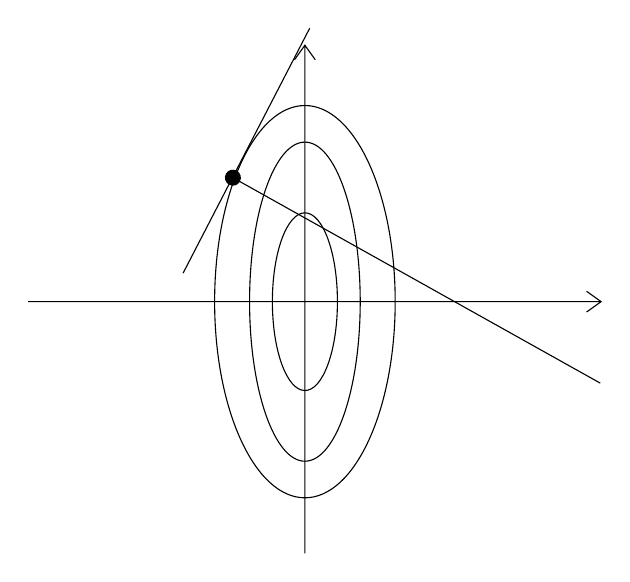
\begin{tikzpicture}[x=0.75pt,y=0.75pt,yscale=-1,xscale=1]
%uncomment if require: \path (0,300); %set diagram left start at 0, and has height of 300

%Shape: Axis 2D [id:dp45343859956492616]
\draw  (153.39,151.55) -- (429.39,151.55)(286.69,28) -- (286.69,272.81) (422.39,146.55) -- (429.39,151.55) -- (422.39,156.55) (281.69,35) -- (286.69,28) -- (291.69,35)  ;
%Shape: Ellipse [id:dp9447732601515546]
\draw   (260.03,151.55) .. controls (260.03,109.1) and (271.97,74.68) .. (286.69,74.68) .. controls (301.41,74.68) and (313.34,109.1) .. (313.34,151.55) .. controls (313.34,194.01) and (301.41,228.42) .. (286.69,228.42) .. controls (271.97,228.42) and (260.03,194.01) .. (260.03,151.55) -- cycle ;
%Shape: Ellipse [id:dp2761663781192929]
\draw   (271.02,151.55) .. controls (271.02,127.91) and (278.03,108.75) .. (286.69,108.75) .. controls (295.34,108.75) and (302.36,127.91) .. (302.36,151.55) .. controls (302.36,175.19) and (295.34,194.36) .. (286.69,194.36) .. controls (278.03,194.36) and (271.02,175.19) .. (271.02,151.55) -- cycle ;
%Shape: Ellipse [id:dp5607371845686238]
\draw   (243.19,151.55) .. controls (243.19,99.36) and (262.66,57.05) .. (286.69,57.05) .. controls (310.71,57.05) and (330.19,99.36) .. (330.19,151.55) .. controls (330.19,203.74) and (310.71,246.05) .. (286.69,246.05) .. controls (262.66,246.05) and (243.19,203.74) .. (243.19,151.55) -- cycle ;
%Straight Lines [id:da9550942603876984]
\draw    (252,91.81) -- (429,190.81) ;
\draw [shift={(252,91.81)}, rotate = 29.22] [color={rgb, 255:red, 0; green, 0; blue, 0 }  ][fill={rgb, 255:red, 0; green, 0; blue, 0 }  ][line width=0.75]      (0, 0) circle [x radius= 3.35, y radius= 3.35]   ;
%Straight Lines [id:da2739448477983437]
\draw    (289,19.81) -- (228,137.81) ;


\end{tikzpicture}

$f(x_k) \approx \left(\dfrac{1 - a}{1 + a}\right)^k$

Идея использовать \textit{"инерцию"}, то есть ранние значения, тогда:

\underline{\textbf{heavyball method (momentum method)}}

$x_{k + 1} = x_k - \alpha_k (\nabla f(x_k) + \beta_kx_{k - 1})$

$f(x_k) = \left(\dfrac{1 - \sqrt{a}}{1 + \sqrt{a}}\right)^k$, что значительно лучше для маленьких $a$.

\end{example}
